\documentclass[11pt]{article}
\usepackage[a4paper,margin=1in]{geometry}
\usepackage[T1]{fontenc}
\usepackage[utf8]{inputenc}
\usepackage{amsmath,amssymb}
\usepackage{graphicx}
\usepackage{hyperref}
\usepackage{enumitem}

\title{X(3872) Three-Body Lineshape: Validation Note}
\author{Misha Mikhasenko \and Contributors}
\date{\today}

\begin{document}
\maketitle

\section*{Summary}
This note validates the three-body phase-space implementation used for the
$\chi_{c1}(3872) \to D^0\bar D^0\pi^0$ and $\chi_{c1}(3872) \to D^0\bar D^0\gamma$
channels in the existing analysis and records the minimal extraction into a
standalone package: \texttt{X3872ThreeBodyLineshape.jl}.

\section*{Implementation status}
\begin{itemize}[leftmargin=1.5em]
    \item Neutral-channel three-body phase space implemented via \texttt{xDDPhaseSpace}.
    \item Minimal API in new package: \texttt{rho\_thr}, \texttt{lineshape}, \texttt{build\_channels}.
    \item Charged-channel constants are placeholders and flagged for later validation.
\end{itemize}

\section*{Validation steps (commands + outputs)}
\begin{itemize}[leftmargin=1.5em]
    \item Ran the notebook to generate the phase-space plots:
\begin{verbatim}
/juliaup/bin/julia --project=.../X3872EffRange.jl -e 'include("notebooks/covariant_rho_thr.jl")'
\end{verbatim}
    \item The plots were produced at:
    \begin{itemize}
        \item \texttt{X3872EffRange.jl/plots/phase\_space\_pi0-gamma.pdf}
        \item \texttt{X3872EffRange.jl/plots/pi0-gamma\_ratio.pdf}
    \end{itemize}
    \item Minor local patch applied for execution:
    \begin{itemize}
        \item add conversion for \texttt{WithThrE} to \texttt{rho\_thr}
        \item guard a Pluto-only cell (\texttt{model\_simpler})
    \end{itemize}
    These are not committed to the source repository.
\end{itemize}

\section*{Plots}
\begin{figure}[h]
    \centering
    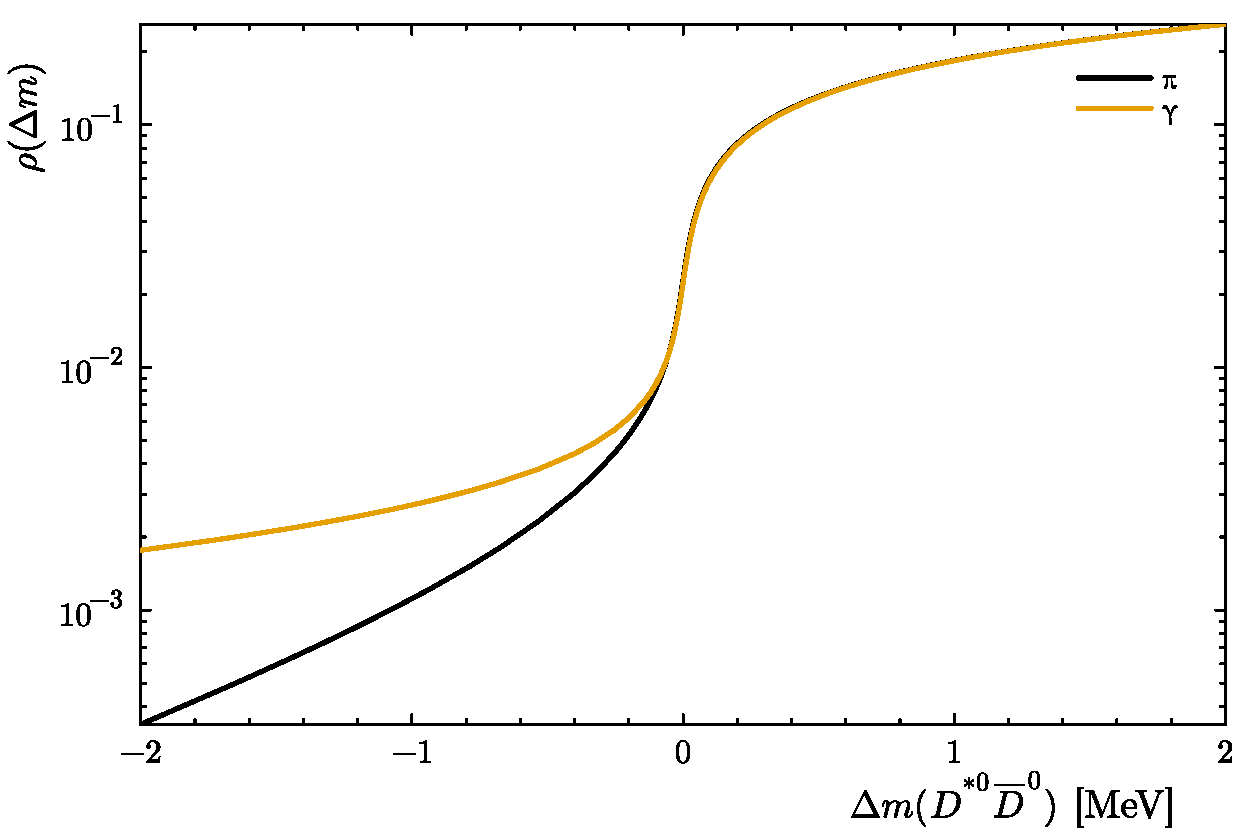
\includegraphics[width=0.8\linewidth]{plots/phase_space_pi0-gamma.pdf}
    \caption{Energy-dependence of the phase-space factors of $\chi_{c1}\to D^0\bar D^0\pi^0$ and $\chi_{c1}\to D^0\bar D^0\gamma$, normalized at $30\,\mathrm{MeV}$ above threshold.}
\end{figure}

\begin{figure}[h]
    \centering
    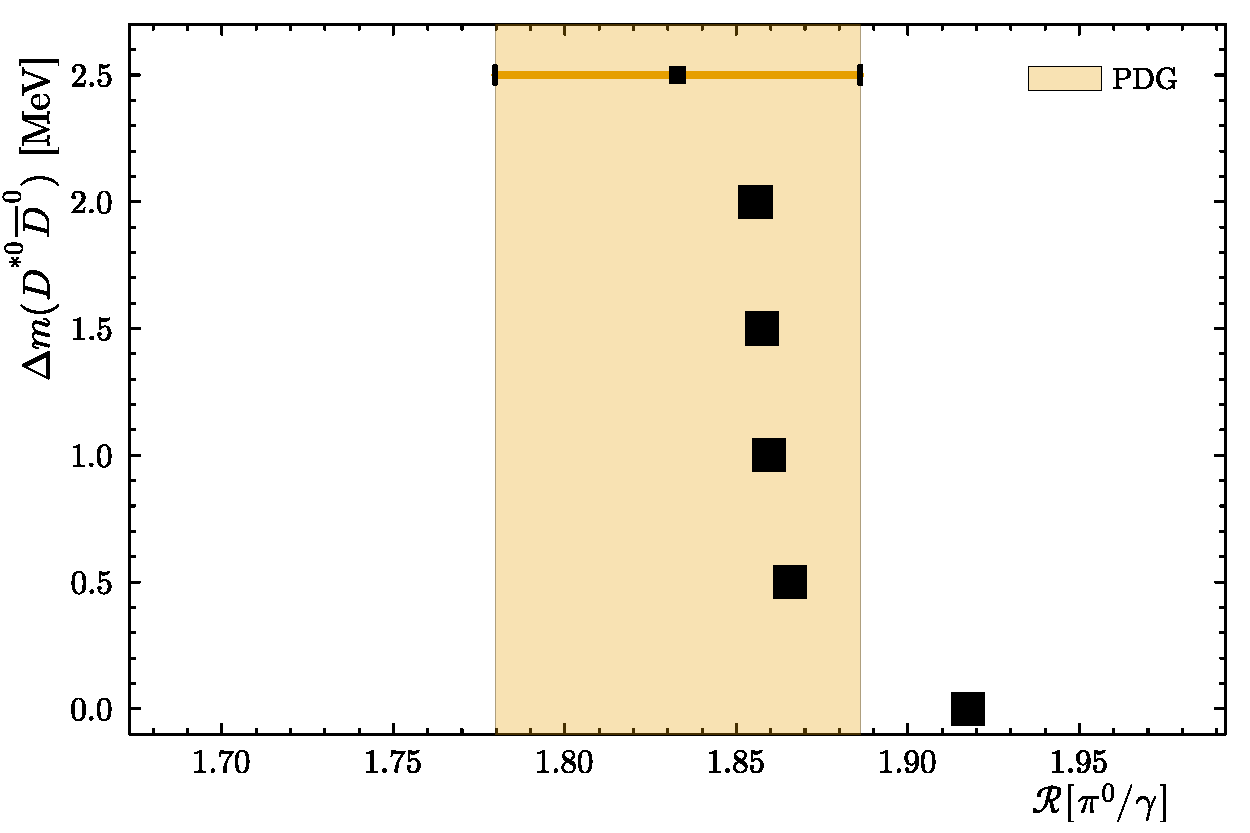
\includegraphics[width=0.8\linewidth]{plots/pi0-gamma_ratio.pdf}
    \caption{Ratio of the phase-space factors for $\chi_{c1}\to D^0\bar D^0\pi^0$ and $\chi_{c1}\to D^0\bar D^0\gamma$. The shaded band corresponds to the PDG branching ratio.}
\end{figure}

\section*{Delta from X3872EffRange}
\begin{itemize}[leftmargin=1.5em]
    \item Extracted a minimal object-based API: \texttt{X3872ThreeBody}, \texttt{denominator}, \texttt{lineshape}, \texttt{rho\_thr}.
    \item Added tests and a parameter table with sources.
    \item Copied validation plots into the new repo for regression reference.
\end{itemize}

\section*{Next}
Iteration 4 adds an analytic-continuation test and a minimal usage example. Iteration 5 updates this note with charged-channel validation once constants are fixed.

\end{document}
